\documentclass{article}
% \usepackage[english]{babel}
% \usepackage[utf8x]{inputenc}

\usepackage{kotex}
\usepackage{graphicx} % Required for inserting images.
\usepackage{geometry}
% \parskip 4.2pt  % Sets spacing between paragraphs.
% \renewcommand{\baselinestretch}{1.5}  % Uncomment for 1.5 spacing between lines.
% \parindent 8.4pt  % Sets leading space for paragraphs.
\usepackage[font=sf]{caption} % Changes font of captions.

\usepackage{amsmath}
\usepackage{amsfonts}
\usepackage{amssymb}
\usepackage{siunitx}
\usepackage{verbatim}
\usepackage{hyperref} % Required for inserting clickable links.
\usepackage{natbib} % Required for APA-style citations.
\usepackage{authblk}

\geometry{
 a4paper,
 left=30mm,
 right=30mm,
 top=30mm,
 bottom=40mm
}

\title{양자 어닐링을 활용한 시간표 생성}
\author[1]{Chae-Hwan Seol}
\author[2]{Si-Won Yun}
\affil[1]{seolchaehwan70@gmail.com}
\affil[2]{yswysw421@gmail.com}

\begin{document}
\maketitle

\begin{abstract}
본 연구는 대표적인 NP-Complete 문제인 시간표 생성 문제를 양자 어닐러(Quantum Annealer)를 활용하여 해결하는 방법을 소개한다. 우선, 생성된 시간표에 대한 비용함수를 도출한다. 비용함수는 적합한 시간표의 조건인 서로 다른 두 시간표에서 동일 시각에 동일한 과목이 배치되었는가, 과목 시간의 수가 적합한가 등에 기반한다. 시간표의 개인화를 위해 부가 조건에 대한 비용함수를 도출한다. 개인화를 위한 조건에는 특정 시간이 연속되는가, 특정 시간이 고정되었는가 등이 존재한다. 도출된 비용함수를 양자 어닐러를 활용하여 실험 사례에 대한 결과를 추출하고 분석을 시행한다. 본 연구에서는 2×3 시간표를 성공적으로 생성하였으며, 양자 어닐링을 활용한 시간표 생성 문제 해결이 가능함을 확인하였다. 그 뿐만 아니라, 본 연구에서 추출된 수식을 활용한 개인화의 가능성 확인을 통해 실생활에 적용 가능함을 확인하였으며, 고전 컴퓨터로 해결이 어려운 NP-Complete 문제를 양자 현상을 활용한 장치를 통해 해결하려는 시도라는 점에서 의의를 가진다.
\end{abstract}

\newpage
\tableofcontents
\newpage

\section{서론}\label{sec:intro}
시간표 생성 문제는 널리 알려진 NP-Complete 문제이다. NP-Complete 문제는 탐색 공간이 너무 넓어 다항 시간 내에 최적해를 찾는 것이 불가하다\cite{kim}. 예컨대 일주일간 총 35시간(하루 7시간씩 5일) 동안 35개의 과목 (중복되지 않는다고 가정)을 배치하는 경우, 한 개의 시간표 생성에 $35!\approx10^{40}$가지 경우의 수를 조사해야 한다.

다른 NP-Complete 문제에는 그래프 색칠 문제가 있다. 그래프 색칠 문제란 특정 개수의 색을 통해 각 변(Edge)에 연결된 서로 다른 두 꼭짓점(Vertex)의 색이 다른 경우를 결정하는 문제이다. 해당 문제는 NP-Complete 문제이기 때문에, 거대한 문제에 대하여 모든 경우의 수를 탐색하는 방법으로 경우를 결정하는 것이 불가하다. 이를 해결하기 위해 휴리스틱적 방법인 양자 어닐링(Quantum Annealing, QA)이 활용되었다.

QA는 양자 터널링 효과(Quantum Tunneling Effect)를 활용하여 해밀토니안(Hamiltonian)이 최저의 에너지 상태를 가지도록 최적화하는 방법이다\cite{kadowaki1998quantum}. 현존하는 D-wave사의 양자 어닐러를 (자세한 정보는 \cite{venegas2018cross}를 참고) 활용하여 시간표 생성 문제를 해결하기 위해서는 문제를 이진(Binary) 변수에 대한 이차 다항식을 최적화하는 문제로 변환해야 한다\cite{tabi2020quantum}. 즉, 조건을 만족하는 경우에서 다항식은 최솟값을 가져야 한다. 이를 QUBO (Quadratic unconstrained binary optimiza-tion)문제라고 한다. 본 연구는 시간표 생성 문제를 QUBO 문제로 변환한 후 양자 어닐러를 활용하여 시간표를 생성하였다.

본 논문의 구성은 다음과 같다. 2장에서는 시간표 생성 문제의 정의와 제약조건을, 3장에서는 각 제약조건을 QUBO 문제로 나타내는 방법을 다룬다. 4장에서는 실제 D-wave 사의 양자 어닐러를 활용한 결과를 분석하며 마지막으론 결론이 뒤따른다.
    
\section{시간표 생성 문제}\label{sec:problem}

시간표 생성 문제는 사용 환경에 따라 다양한 부속 조건의 설정이 가능하다. 즉 문제를 다양하게 정의 가능하기에 명확한 문제 정의가 필요하다. 본 연구에서는 시간표 생성 문제를 다음과 같이 정의한다.

    \paragraph{시간표 생성 문제의 정의}
    \begin{enumerate}
        \item 시간표는 학생 개개인을 대상으로 생성한다. 즉 각 학생은 서로 다른 시간표를 배정받는다.
        \item 시간표에 각 시간에 대한 과목은 제약 조건에 만족하는 과목으로 구성된다. (제약 조건은 아래에서 자세히 다룬다.)
    \end{enumerate}

본 논문에서는 2가지의 강한 제약 조건과 2가지의 약한 제약 조건을 설정하였다. 강한 제약 조건은 합당한(물리적, 시간적으로 모순 없는) 시간표 생성을 위한 조건이다. 약한 제약 조건은 사용자가 원하는 문제 상황을 정의 및 설정하기 위한 조건이다. 이는 강한 제약 조건과 다르게 필수적이지 아니하다.

    \paragraph{강한 제약 조건}
    \begin{enumerate}
        \item 한 명의 강사는 동일 시간에 하나의 장소에서만 강의할 수 있다. 즉 한 명의 강사는 동일 시간 동일 장소에서 강의하는 것이 불가하다.
        \item 각 과목은 한 주당 수업 시수가 정해져 있다. 즉 각 과목은 정해진 수업 시수를 초과하거나 부족하면 아니된다.
    \end{enumerate}

    \paragraph{약한 제약 조건}
    \begin{enumerate}
        \item 특정 과목은 이어 진행한다(연강).
        \item 특정 과목은 설정한 시간에 강의가 진행된다(위치 지정).
    \end{enumerate}
    
본 연구에서는 2명의 학생에 대한 $3\times2$ 크기의 시간표 생성을 실험하였다. 

\section{본론}\label{sec:main}

\subsection{변수 표기법}

시간표 생성 문제를 QUBO 문제로 표현하기 위한 수식에 사용되는 변수 표기법을 정의해야 한다.

    \begin{equation}\label{eqn:variable1}
        x_{t,x,y,m}
    \end{equation}

각 변수는 (\ref{eqn:variable1})과 같이 표현되며, 0 또는 1의 값을 가진다. 변수의 아래 첨자는 다음을 의미한다. Figure \ref{fig:variable}은 변수 표기법에 따라 나타낸 그림이다.

    \begin{enumerate}
        \item [] $t$: 시간표의 사용자(학생)
        \item [] $x,y$: 시간표에서 위치
        \item [] $m$: 과목을 나타내는 이진수 코드의 자릿수
    \end{enumerate}

    \begin{figure}[htb!]
        \centering
        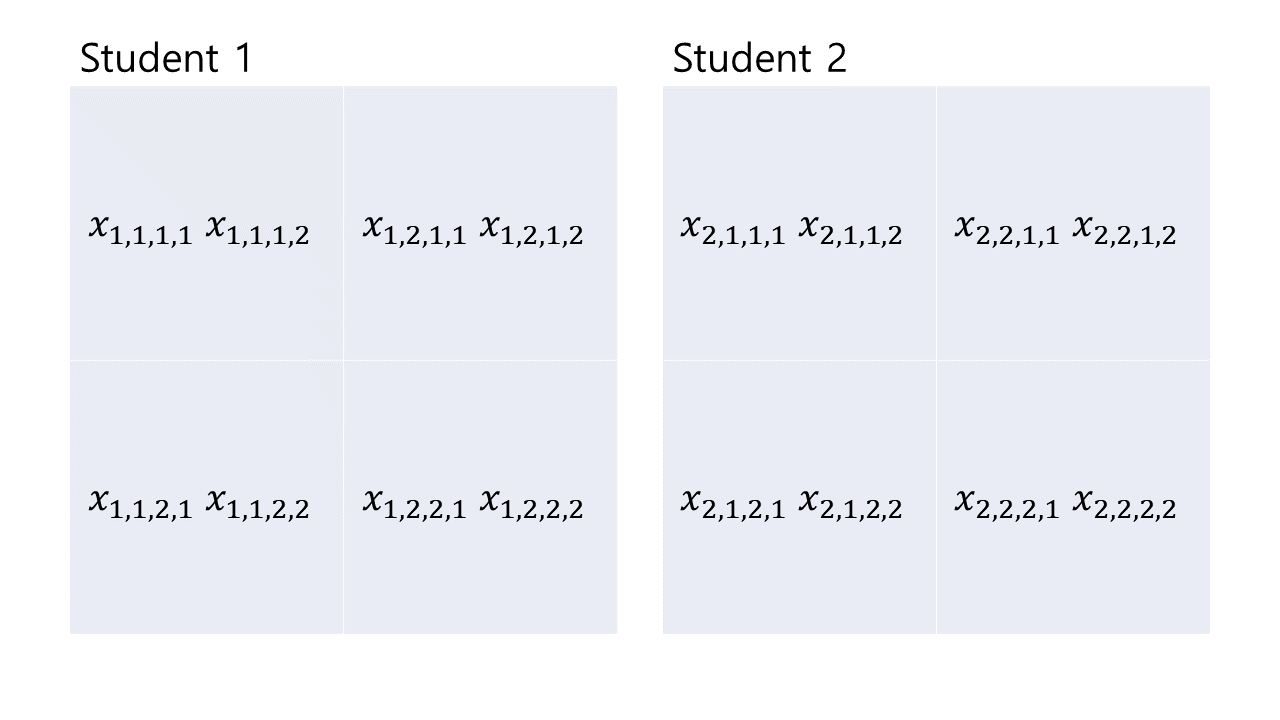
\includegraphics[width=0.8\columnwidth]{images/var1.png}
        \caption{2명의 학생에 대해 $2 \times 2$ 크기의 시간표를 만들 때 변수 표기법}
        \label{fig:variable}
    \end{figure}

각 과목은 이진수 코드를 할당한다. 예를 들어, 3자리 이진수를 코드로 할당할 경우, $2^{3}=8$개의 과목을 표현할 수 있으며 수학은 100, 물리는 010, 화학은 110과 같이 나타낼 수 있다. 각 과목은 식을 생성하는 단계에서 사용자가 필요에 따라 설정한다.

    \subsection{강한 제약 조건}

첫번째 강한 제약 조건은 한 명의 강사는 동일 시간에 하나의 장소에서만 강의할 수 있다는 것이다. 두개의 시간표 $t_{i}$와 $t_{j}$의 (x,y) 시간을 비교하기 위해 아래의 수식 (\ref{eqn:strong1})를 활용한다.

    \begin{equation}\label{eqn:strong1}
        \prod_{b=1}^{bit}((1-x_{t_{i},x,y,b} )(1-x_{t_{j},x,y,b})+x_{t_{i},x,y,b} x_{t_{j},x,y,b} )
    \end{equation}

수식 (\ref{eqn:strong1})는 두개의 시간표의 동일 시간에서 과목이 같다면 1, 아니면 0을 출력한다. 다른 수업을 들어야 하는 학생의 시간표를 생성할 경우 수식 (\ref{eqn:strong1})를 적용한다. 공강 시간의 경우 다른 시간표와 겹치더라도 문제가 되지 않는데, 이 경우, 아래 수식 (\ref{eqn:strong2})을 추가로 곱하여 해결 가능하다. $q_{i}$는 공강 시간에 배정된 이진수 코드의 i번째 자리를 의미한다. 예컨대, 공강 시간을 000으로 설정할 경우 모든 $q_{i}$는 0이다.

    \begin{equation}\label{eqn:strong2}
        \prod_{b=1}^{bit}(1-((1-x_{t_{i},x,y,b} )(1-x_{t_{j},x,y,b} )(1-q_{b} )+ x_{t_{i},x,y,b}\times x_{t_{j},x,y,b} \times q_{b} )) 
    \end{equation}

두번째 강한 제약 조건은 각 과목이 한 주당 수업 시수가 정해져 있다는 것이다. 수식 (\ref{eqn:strong3})는 한 시간표의 모든 시간에 대해 특정 과목(하나의 과목)과 동일한 과목인지 비교한 후 결과의 합을 출력한다. 수식 (\ref{eqn:strong3})의 $T_{i}$는 수식 (\ref{eqn:strong2})의 $q_{i}$와 유사하게 특정 과목을 표현하는 이진수 코드의 i번째 자리를 의미한다. 이후 특정 과목의 설정된 시수와 차를 제곱하는 형태이다.

    \begin{equation}\label{eqn:strong3}
        \left( \sum_{every\;x,y} \left( \prod_{b=1}^{bit}((1-x_{t_{i},x,y,b} )(1-x_{t_{j},x,y,b} )(1-T_{b})+x_{t_{i},x,y,b} x_{t_{j},x,y,b} T_{b} ) \right) -(number\;of class)\right )^{2}
    \end{equation}

    \subsection{약한 제약 조건}

첫번째 약한 제약 조건, 연강은 특정 과목은 이어 진행한다, 즉 연강으로 진행한다는 것이다. 연강과 관련된 수식은 아래와 같다. 

    \begin{equation}\label{eqn:weak1}
        \prod_{b=1}^{bit} \left( \left( \prod_{e=0}^{time-1}x_{t,x,y+e,b} \right) q_{b}+\left ( \prod_{e=0}^{time-1} (1-x_{t,x,y+e,b}) \right) (1-q_{b}) \right ) 
    \end{equation}

위에 수식 (\ref{eqn:weak1})에서 $q_{i}$는 연강으로 진행할 과목의 $i$번째 자리를 의미한다. $time$은 설정된 연강 시간을 의미한다. 예컨대 화학 과목이 연강이며, $time=3$일 경우 화학 과목은 세시간 연속하여 배치된다. 위 수식 (\ref{eqn:weak1})는 특정 좌표부터, $time$개의 시간이 목표 과목(연강 과목)과 동일할 경우 1, 아니면 0을 출력한다. 우리가 구하고자 하는 함수는 비용 함수이므로, 조건을 만족할 때 최솟값(0)을 가져야 한다. 또한, 시간표의 특정 열에 대하여 연강의 조건을 만족할 경우 시간표에 연강이 존재하는 것으로 판단한다. 따라서, 연강과 관련된 비용함수는 개인의 시간표에서 모든 열에 대하여 연강이 존재하지 않을 경우 1을, 한 열이라도 연강이 존재할 경우 0을 출력한다. 각 열에 대하여 수식 (\ref{eqn:weak1})의 $y$의 값은 개인 시간표에 적합한 범위를 대입한다. 즉, $1 \leq y \leq (Size of Row)-(time)+1$를 만족하는 모든 정수의 y 값을 대입한다. 요컨대, 대입하여 제작된 수식 중 1이 존재할 경우 해당 열에는 연강이 존재한다.

    두번째 약한 제약 조건, 위치 지정은 특정 과목(목표 과목)이 설정된 시간에 강의가 진행된다는 것이다. 해당 약한 제약 조건을 위한 수식은 아래와 같다.

    \begin{equation}\label{eqn:weak2}
        1- \prod_{b=1}^{bit}\left ( (1-x_{t_{i},x,y,b} )(1-q_{b} )+x_{t_{i},x,y,b} q_{b} \right ) 
    \end{equation}

    \begin{equation}\label{eqn:weak3}
        \prod_{b=1}^{bit}\left ( (1-x_{t_{i},x,y,b} )(1-q_{b} )+x_{t_{i},x,y,b} q_{b} \right ) 
    \end{equation}

위에 수식 (\ref{eqn:weak2})에서 $q_{i}$는 수식 (\ref{eqn:strong2})에서의 사용과 용도 및 의미가 일치한다. 수식 (\ref{eqn:weak2})은 목표 과목과 위치 $x$,$y$가 가리키는 시간의 과목이 같다면 0을 출력한다. 해당 식을 활용하여 약한 제약 조건에 맞지 않을 경우 비용 함수 값을 증가시킬 수 있다. 수식 (\ref{eqn:weak2})을 수식 (\ref{eqn:weak3})과 같이 변형하여 특정 과목이 특정한 시간에 배치되는 것을 피할 수 있다. 수식 (\ref{eqn:weak3})은 수식 (\ref{eqn:weak2})의 비트를 반전시켜 목표 과목과 위치 $x$,$y$가 가리키는 시간의 과목이 같지 않을 때 0을 출력한다.

    \subsection{Degree Reduction}

앞선 과정을 통해 생성된 수식은 이차 이상의 차수를 가질 가능성이 존재한다. 서론에서 언급한 바와 같이 양자 어닐링을 위해 수식을 이차 다항식으로 변환할 필요가 있다(수식의 차수를 낮추어야 한다). 수식의 차수는 Degree Reduction 기법을 활용하여 낮춘다. Degree Reduction 기법을 통해 변환된 수식은 기존 다항식과 최솟값을 가지는 변수 조합이 일치하여야 한다. 더 정확하게 말하면, 기존 다항식 $p$가 변수 집합 $X=\{x_{0},\cdot,x_{i} \}$에서 최솟값을 가질 때, 변환된 수식 $q$ 또한 변수 집합 X와 Degree Reduction 과정에서 추가로 생기는 변수 집합 $W=\{w_{0},\cdot,w_{m} \}$에서 최솟값을 가진다.

Degree Reduction은 경우에 따라 Freedman의 방법 또는 Ishikawa의 방법을 활용한다. Freedman의 방법을 활용할 경우 계수가 음수인 단항식을 이차식으로 변환할 수 있으며\cite{freedman2005energy}, Ishikawa의 방법을 활용하면 계수가 양수인 단항식을 이차식으로 변환할 수 있다. \cite{ishikawa2010transformation} Freedman의 방법은 항 $-x_{1}\cdot x_{m} (m>2)$을 항 $w_{1} (d-1-\sum_{i=1}^{d}x_{i} )$로 변환한다. Ishikawa의 방법은 항 $x_{1}\cdot x_{m} (m>2)$에서 $m$이 짝수일 경우 수식 (\ref{eqn:ishikawa1})을 통해, $m$이 홀수일 경우 수식 (\ref{eqn:ishikawa2})를 통해 항을 변환한다. $w_{1},\cdot,w_{k}$는 Degree Reduction 과정을 통해 새롭게 생성된 변수이며, 다른 변수와 동일하게 0 또는 1의 값을 가진다. 수식 (\ref{eqn:ishikawa1})과 수식 (\ref{eqn:ishikawa2})에서 $k = \lfloor (m-1)\/2 \rfloor$이다. 

    \begin{equation}\label{eqn:ishikawa1}
        \sum_{i<j}x_{i}  x_{j}+\sum_{j=1}^{k}(4j-1) w_{j} -2\left( \sum_{j=1}^{k}w_{j} \right) \left ( \sum_{j=1}^{m}x_{j} \right )
    \end{equation}

    \begin{equation}\label{eqn:ishikawa2}
            \sum_{i<j}x_{i}  x_{j}+\sum_{j=1}^{k} (4j-1) w_{j} - 2\left ( \sum_{j=1}^{k}w_{j} \right) \left(\sum_{j=1}^{m}x_{j} \right)+w_{k} \left (\sum_{j=1}^{m}x_{j} -m+1\right )
    \end{equation}

    \subsection{구현 방법}

프로그래밍 언어 Python의 3.10 버전을 활용하여 수식 생성 프로그램을 제작하였다. 수식의 생성을 위해 Python의 sympy model을 활용하였으며, 생성된 시간표의 시각화를 위해 Python의 matplotlib model을 활용하였다. 

    \section{결과}

    \subsection{실험 사례 분류}

실험 사례에 대한 적합한 시간표 생성 확인을 통해 양자 어닐링을 활용한 시간표 생성 문제 해결이 가능함을 검증하였다. 모든 실험 사례는 앞서 언급하였던 바와 같이 $2\times3$ 크기의 2학생에 대한 시간표로 정의한다. 각 제약 조건에 대한 검증을 위하여 총 6가지 실험 사례를 준비하였다. 아래 표 (\ref{tab:kindofcase})에 각 실험 사례의 조건을 정리하였다.

    \begin{table}[htb!]
        \centering
        \begin{tabular}{ c c c c c }
        \hline
        \begin{tabular}{c}
          실험 사례\\
          번호
        \end{tabular}&
        \begin{tabular}{c}
          공강 적용\\
          여부
        \end{tabular}&
        \begin{tabular}{c}
          연강 적용\\
          여부
        \end{tabular}&
        \begin{tabular}{c}
          위치 지정\\
          여부
        \end{tabular}&
        \begin{tabular}{c}
          시간표 생성\\
          가능 여부
        \end{tabular}\\
        \hline
        1 & X & X & X & O \\
        2 & O & X & X & O \\
        3 & X & O & X & O \\
        4 & X & X & O & O \\
        5 & X & O & O & O \\
        6 & X & O & X & X \\
        \hline
        \end{tabular}
        \caption{실험 사례 조건}\label{tab:kindofcase}
    \end{table}

모든 실험 사례는 강한 제약 조건이 적용된다. 약한 제약 조건은 사용자가 원하는 문제 상황 정의 및 설정을 위해 활용되어, 각 실험 사례에서 약한 제약 조건을 설정하여 문제 상황을 정의하였다.

1번 실험 사례는 강한 제약 조건의 작동 여부를 검증한다. 약한 제약 조건을 설정하지 않아 강한 제약 조건에 대한 검증이 가능하다. 2, 3, 4번 실험 사례는 각각 공강, 연강, 위치 지정의 작동 여부를 검증한다. 5번 실험 사례는 약한 제약 조건을 중복으로 설정할 경우의 작동 여부를 검증한다. 6번 실험 사례는 해결이 불가능한 문제와 해결이 가능한 문제를 비교하기 위해 진행하였다.

    \subsection{실험 환경}

모든 실험 사례에 대하여 본 논문에서 소개하는 방법을 통해 수식을 생성하고 D-wave사의 양자 어닐러를 활용하여 실험을 진행하였다. 각 실험 사례에 대하여 10번씩 실험을 진행하였으며, 각 실험은 양자 어닐러를 1000번 돌려 나온 최적값을 출력한다.

    \subsection{변수 표기법}

표현의 간편화를 위하여 새로운 변수 표기법을 정의한다.

    \begin{equation}\label{eqn:newvar}
        v_{i}
    \end{equation}

기존 변수 표기법과 달리 새로운 변수 표기법의 경우 아래 첨자에 1개의 변수만이 존재한다. $i$는 아래 수식(\ref{eqn:howtoi})을 활용하여 구할 수 있다.

    \begin{equation}\label{eqn:howtoi}
        tWHB+(xH+y)B+m-1
    \end{equation}

변수 $t$,$x$,$y$,$m$은 앞선 변수 표기법에서의 변수 $t$,$x$,$y$,$m$와 의미가 같다.

    \begin{enumerate}
        \item [] $t$: 시간표의 사용자(학생)
        \item [] $x,y$: 시간표에서 위치
        \item [] $m$: 과목을 나타내는 이진수 코드의 자릿수
    \end{enumerate}

상수 $W$,$H$,$N$,$B$는 생성하고자 하는 시간표의 설정 값이다. 즉 모든 표기하는 모든 변수에 대하여 동일한 값을 가지는 상수이다. 각각의 의미는 아래와 같다.

    \begin{enumerate}
        \item [] $W,H$: 생성할 시간표의 가로, 세로 길이
        \item [] $N$: 생성할 시간표의 개수
        \item [] $B$: 과목을 나타내기 위해 사용하는 비트 수
    \end{enumerate}

따라서 시간표를 생성하는데 필요한 변수의 개수는 수식 (\ref{eqn:numberofvar})을 통해 구할 수 있다.

    \begin{equation}\label{eqn:numberofvar}
        WHNB
    \end{equation}

Figure \ref{fig:variable}는 그림 \ref{fig:variable}의 시간표 변수를 새로운 표기법으로 바꾸어 표시한 그림이다.

    \begin{figure}[htb!]
        \centering
        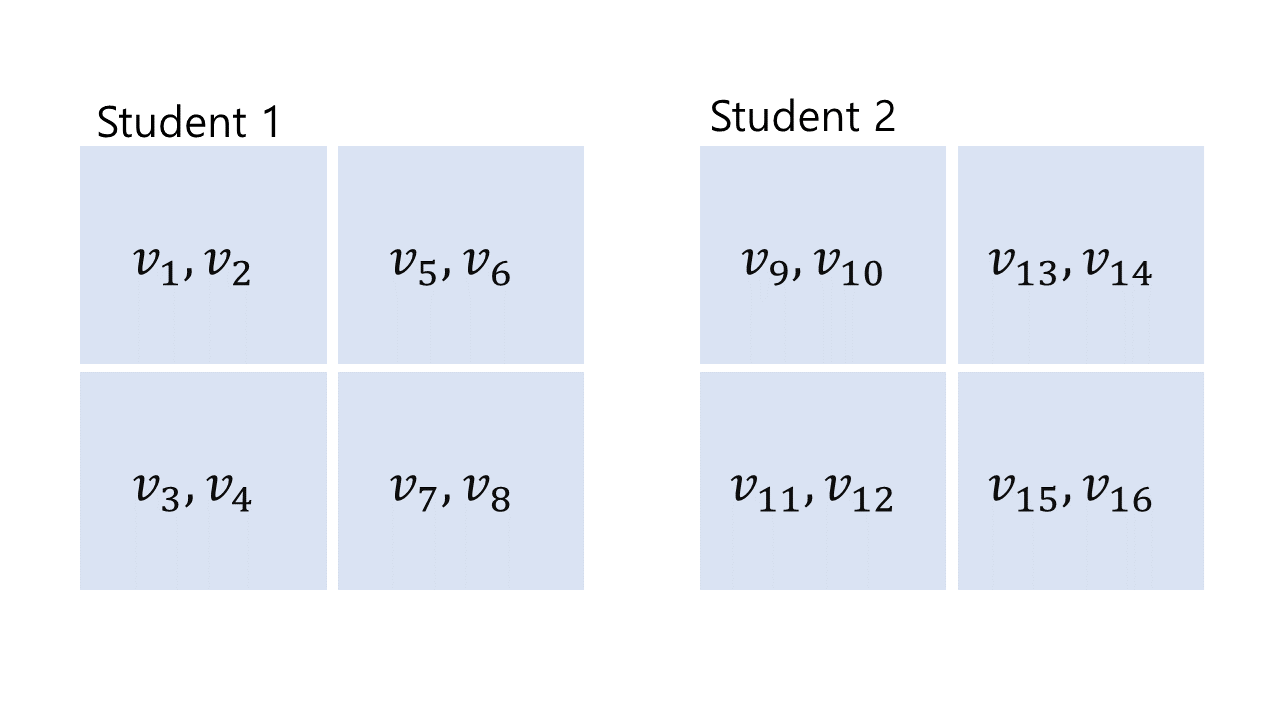
\includegraphics[width=0.8\columnwidth]{images/var2.png}
        \caption{2명의 학생에 대해 $2 \times 2$ 크기의 시간표를 만들 때 변수 표기법}
        \label{fig:newvar}
    \end{figure}

    \subsection{실험}

아래 실험 사례에서는 언급하지 않았으나 모든 실험 사례에서 실행시간은 1초 미만이었다. 즉, 식이 생성되어 있는 경우, 양자 어닐러를 통해 답을 얻어내는 과정은 빠르게 여러 번 시행해볼 수 있다.

    \subsubsection{실험 사례 1 - 강한 제약 조건}

본 실험 사례에서는 강한 제약 조건에 대하여 실험한다. 해당 실험 사례에는 3가지 과목이 존재한다. 각 과목은 2비트를 활용하여 표현하였다. 각 과목에 대한 설정은 Table \ref{tab:testcase1}와 같다.

    \begin{table}[htb!]
        \centering
        \begin{tabular}{c c c}
             \hline
             과목 이름 & 수업 시수 & 과목 표현 코드\\
             \hline
             A & 2 & 00 \\
             B & 2 & 10 \\
             C & 2 & 01 \\
             \hline
        \end{tabular}
        \caption{실험 사례 1의 설정값}\label{tab:testcase1}
    \end{table}

위 실험 사례를 본 연구에서 다루는 방법을 활용하여 양자 어닐링을 실행한 결과 출력된 변수 값은 \ref{results}. 부록의 Table \ref{tab:result1}에 나열하였다. Case 1뿐만 아니라 모든 실험의 결과에서 Degree reduction 과정에서 생기는 추가적인 변수의 결과값은 중요한 값이 아니며, 개수가 많아 표현하기에 한계가 있어 생략하였다.

Figure \ref{fig:case1}은 10번째 실험에서 출력된 변수 값에 기반하여 시각화 된 시간표이다. Figure \ref{fig:case1}과 같이 두 시간표에 겹치는 부분이 없고, A, B, C 과목은 설정한 값과 같이 각각 2시간씩 배정되었다. 강한 제약 조건이 의도한 바와 같이 적용되어 10번의 실험에서 모두 Cost가 0이다.

    \begin{figure}[htb!]
        \centering
        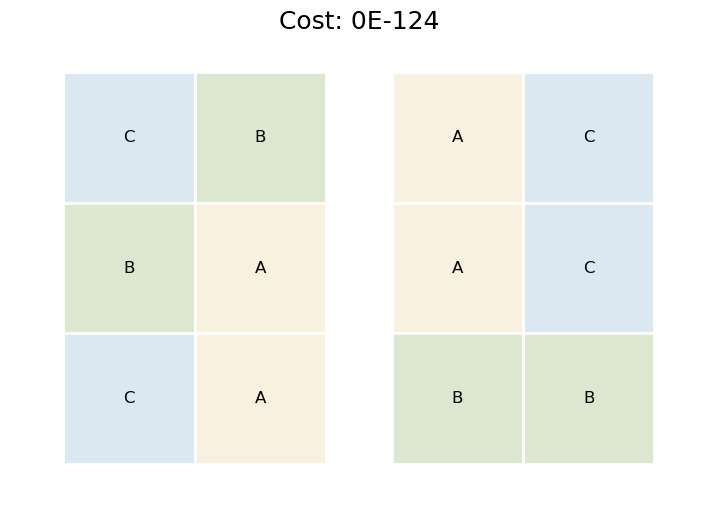
\includegraphics[width=0.6\textwidth]{images/Case1.png}
        \caption{실험 사례 1의 10번째 결과}
        \label{fig:case1}
    \end{figure}

    \subsubsection{실험 사례 2 - 공강}

본 실험 사례에서는 약한 제약 조건 중 공강에 대하여 실험한다. 각 과목에 대한 설정은 Table \ref{tab:testcase2}과 같다.

    \begin{table}[htb!]
        \centering
        \begin{tabular}{c c c c}
             \hline
             과목 이름 & 수업 시수 & 과목 표현 코드 & 공강 여부\\
             \hline
             A & 1 & 00 & X\\
             B & 1 & 10 & X\\
             Free & 4 & 01 & O\\
             \hline
        \end{tabular}
        \caption{실험 사례 2의 설정값}\label{tab:testcase2}
    \end{table}

free 과목은 공강으로 설정되어 있다. 공강을 4시간 부여함으로써 공강이 필연적으로 동일 시간에 배치되는 상황을 설정하였다. 양자 어닐링을 실행한 결과 출력된 변수 값은 \ref{results}. 부록의 Table \ref{tab:result2}에 나열하였다.

Figure \ref{fig:case2}는 10번째 실험에서 출력된 변수 값에 기반하여 시각화 된 시간표이다. 그림 Figure \ref{fig:case2}의 시간표는 강한 제약 조건을 모두 만족시켰고, 공강으로 설정한 free과목은 두 시간표에서 겹치고 있지만 Cost가 0이 되며 올바른 시간표를 생성한 것을 확인할 수 있다.

    \begin{figure}[htb!]
        \centering
        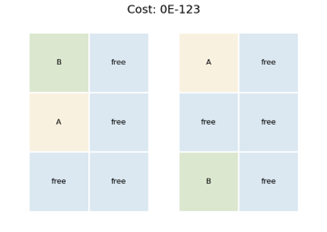
\includegraphics[width=0.6\textwidth]{images/Case2.png}
        \caption{실험 사례 2의 10번째 결과}
        \label{fig:case2}
    \end{figure}

    \subsubsection{실험 사례 3 - 연강}

본 실험 사례에서는 약한 제약 조건 중 연강에 대하여 실험한다. 각 과목에 대한 이름 및 수업 시수, 과목 표현 코드는 실험 사례 1과 동일하지만, 해당 실험 사례에서는 A 과목이 2시간 연강으로 설정하였다. 양자 어닐링을 실행한 결과 출력된 변수 값은 \ref{results}. 부록의 Table \ref{tab:result3}에서 확인할 수 있다.

    \begin{table}[htb!]
        \centering
        \begin{tabular}{c c c c}
             \hline
             과목 이름 & 수업 시수 & 과목 표현 코드 & 연강\\
             \hline
             A & 2 & 00 & 2\\
             B & 2 & 10 & 0\\
             C & 2 & 01 & 0\\
             \hline
        \end{tabular}
        \caption{실험 사례 3의 설정값}\label{tab:testcase3}
    \end{table}

Figure \ref{fig:case3}는 9번째 실험(Cost: 0)에서 출력된 변수 값에 기반하여 시각화 된 시간표이다. 만들어진 시간표에서 A 시간이 연속하여 배치된 결과를 확인할 수 있다. Table \ref{tab:result3}에선 일부 경우에서 Cost 값은 0이다. 그러나 다수의 경우에서 Cost 값은 1 또는 2이다. 

    \begin{figure}[ht]
        \centering
        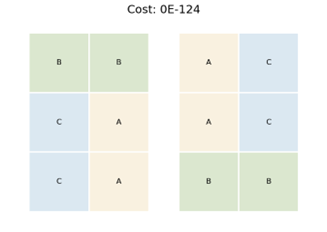
\includegraphics[width=0.6\textwidth]{images/Case3.png}
        \caption{실험 사례 3의 9번째 결과}
        \label{fig:case3}
    \end{figure}
    \newpage  % 임시....

    \subsubsection{실험 사례 4 - 위치 지정}

본 실험 사례에서는 약한 제약 조건 중 위치 지정에 대하여 실험한다. 각 과목에 대한 이름 및 수업 시수, 과목 표현 코드는 실험 사례 1과 동일하며 A 과목의 위치를 지정하였다. 아래 Table \ref{tab:testcase4}에서 위치 (x,y)는 시간표의 x번째 행, y번째 열을 의미한다.

    \begin{table}[htb!]
        \centering
        \begin{tabular}{c c c c c}
             \hline
             과목 이름 & 수업 시수 & 과목 표현 코드 & 위치 지정 & 금지 위치 지정\\
             \hline
             A & 2 & 00 & 
             \begin{tabular}{@{}l@{}}
                  Student1:(3,1) \\
                  Student2:(3,2)
             \end{tabular}
             &
             \begin{tabular}{@{}l@{}}
                Student1:(3,2)\\
                Student2:(3,1)
             \end{tabular}\\
             B & 2 & 10 & None & None\\
             C & 2 & 01 & None & None\\
             \hline
        \end{tabular}
        \caption{실험 사례 4의 설정값}\label{tab:testcase4}
    \end{table}

양자 어닐링을 실행한 결과 출력된 변수 값은 \ref{results}. 부록의 Table \ref{tab:result4}을 통해 확인할 수 있다.

Figure \ref{fig:case4}은 10번째 실험에서 출력된 변수 값에 기반하여 시각화 된 시간표이다. 

    \begin{figure}[htb!]
        \centering
        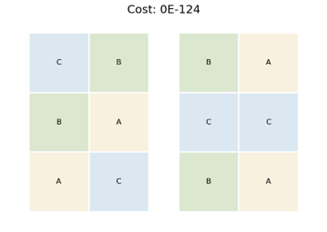
\includegraphics[width=0.6\textwidth]{images/Case4.png}
        \caption{실험 사례 4의 10번째 결과}
        \label{fig:case4}
    \end{figure}

A 과목은 첫번째 시간표에서 위치 (3,1), (2,2)에, 두번째 시간표에서는 위치 (1,2), (3,2)에 배치되었다. 이는 설정 값을 만족하며, 위치 지정 약한 제약 조건이 의도한 바와 같이 작동함을 확인할 수 있다. 또한 Cost 값은 모두 0이다.

    \subsubsection{실험 사례 5 - 연강 및 위치 지정}

본 실험 사례에서는 약한 제약 조건 중 연강과 위치 지정을 중복하여 활용한다. A 과목을 2시간 연강으로 설정하였으며, 위치를 지정하였다.

    \begin{table}[htb!]
        \centering
        \begin{tabular}{c c c c c}
             \hline
             과목 이름 & 수업 시수 & 과목 표현 코드 & 연강 & 위치 지정\\
             \hline
             A & 2 & 00 & 2 & Student1:(3,1) Student2:(3,2)\\
             B & 2 & 10 & 0 & None\\
             C & 2 & 01 & 0 & None\\
             \hline
        \end{tabular}
        \caption{실험 사례 5의 설정값}\label{tab:testcase5}
    \end{table}

양자 어닐링을 실행한 결과 출력된 변수 값은 \ref{results}. 부록의 Table \ref{tab:result5}에 나열하였다. Figure \ref{fig:case5}은 9번째 실험(Cost: 0)에서 출력된 변수 값에 기반하여 시각화 된 시간표이다.

    \begin{figure}[htb!]
        \centering
        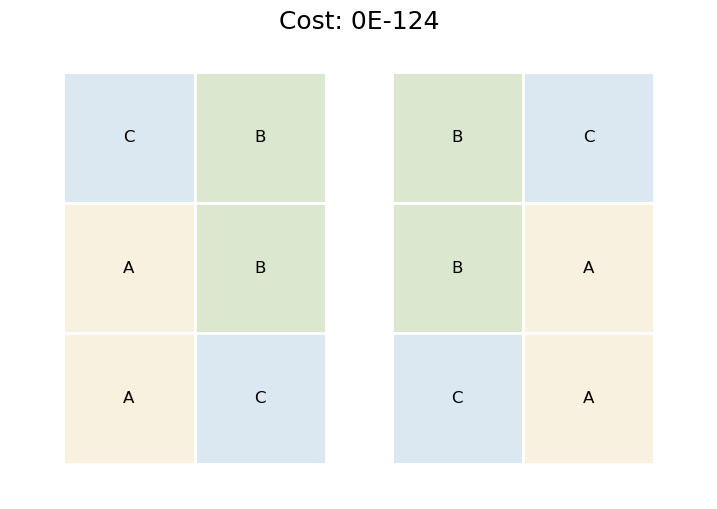
\includegraphics[width=0.6\textwidth]{images/Case5.png}
        \caption{실험 사례 5의 9번째 결과}
        \label{fig:case5}
    \end{figure}

연강으로 설정된 A과목이 연달아 잘 배치되며, 동시에 위치도 의도한 바와 같이 지정되었다. Case 3의 경우와 같이 Cost 값이 0인 경우가 존재하나, 다수의 경우 Cost의 값은 2이다. 

    \subsubsection{실험 사례 6 - 생성이 불가능한 경우}

본 실험에서 각 과목에 대한 설정은 Table \ref{tab:testcase6}과 같다. 과목 A와 B가 연강과 위치 지정을 동시에 만족할 수 없는 경우를 통해 나온 결과는 \ref{results}. 부록의 Table \ref{tab:result6}에 나열하였다. 이 경우에는 10번의 실험 모두 Cost가 0보다 커지면서 시간표가 생성되지 않는 결과가 의도한 바와 같이 나왔다. 

    \begin{table}[htb!]
        \centering
        \begin{tabular}{c c c c c}
             \hline
             과목 이름 & 수업 시수 & 과목 표현 코드 & 연강 & 위치 지정\\
             \hline
             A & 2 & 00 & 2 & Student1:(3,1) Student2:(3,2)\\
             B & 2 & 10 & 2 & Student1:(1,1) Student2:(1,2)\\
             C & 2 & 01 & 0 & None\\
             \hline
        \end{tabular}
        \caption{실험 사례 6의 설정값}\label{tab:testcase6}
    \end{table}

    \section{결론}

본 연구에서는 대표적인 NP-complete 문제인 시간표 생성 문제를 양자 어닐러를 활용하여 해결하는 방법을 제안한다. 이를 위해 올바른 시간표가 갖추어야 할 제약 조건들을 설정하고, 해당 조건을 식으로 표현하였다. 제안한 방법의 검증을 위해 학생 2명의 $2\times3$크기 시간표를 생성하는 경우에 대하여 세부 조건을 조작하였으며, D-wave사의 양자 어닐러를 활용하여 각각 10번씩 실험하였다.

그 결과 물리적으로 시간표 생성이 불가한 경우를 제외하곤 생성한 식의 최솟값이 0인 경우를 1초 내외로 찾아내었다. 그러나, 연강을 적용한 경우, 모든 경우에서 최솟값을 찾지는 못하였다. 이의 원인은 양자 어닐링 과정에서 여러 에너지 상태를 동시에 가질 수 있기에 발생할 것으로 추측된다. 최소 에너지와 다른 에너지 사이의 간격이 작은 경우 어닐링 과정에서 최소 에너지를 찾기 못할 수도 있다.

본 연구에서 양자 어닐링을 활용하여 시간표 생성이 가능하다는 것을 확인하였다. 실생활에 사용되기 위해선 연강 조건을 설정하는 식을 새롭게 찾아내거나 계수를 수정하는 방식으로 에너지 틈이 좁아 생기는 문제를 해결하는 연구가 진행되어야 한다.

    \newpage
    \bibliographystyle{unsrt}
    \bibliography{refs}
    
    \newpage

    \appendix
    \section{실험 결과}\label{results}

    \begin{table}[htb!]
    \small
    \begin{minipage}{0.475\linewidth}
%     \centering
    \begin{tabular}{c | c c c c c c c c c c}
        \hline
        value & 1 & 2 & 3 & 4 & 5 & 6 & 7 & 8 & 9 & 10 \\
        \hline
        $v_0$ & 0 & 1 & 0 & 0 & 0 & 0 & 0 & 0 & 0 & 0 \\
        $v_1$ & 1 & 0 & 0 & 1 & 1 & 1 & 0 & 0 & 1 & 1 \\
        $v_2$ & 1 & 0 & 1 & 0 & 1 & 0 & 0 & 0 & 1 & 1 \\
        $v_3$ & 0 & 1 & 0 & 0 & 0 & 0 & 1 & 0 & 0 & 0 \\
        $v_4$ & 0 & 0 & 0 & 1 & 1 & 1 & 0 & 1 & 1 & 0 \\
        $v_5$ & 0 & 1 & 1 & 0 & 0 & 0 & 0 & 0 & 0 & 1 \\
        $v_6$ & 0 & 0 & 0 & 1 & 0 & 0 & 1 & 0 & 0 & 1 \\
        $v_7$ & 0 & 0 & 1 & 0 & 1 & 1 & 0 & 1 & 1 & 0 \\
        $v_8$ & 0 & 0 & 1 & 0 & 0 & 0 & 0 & 0 & 0 & 0 \\
        $v_9$ & 1 & 0 & 0 & 1 & 0 & 0 & 1 & 1 & 0 & 0 \\
        $v_{10}$ & 1 & 1 & 0 & 0 & 1 & 1 & 1 & 1 & 0 & 0 \\
        $v_{11}$ & 0 & 0 & 0 & 0 & 0 & 0 & 0 & 0 & 0 & 0 \\
        $v_{12}$ & 0 & 0 & 1 & 1 & 1 & 1 & 0 & 0 & 1 & 0 \\
        $v_{13}$ & 0 & 0 & 0 & 0 & 0 & 0 & 1 & 1 & 0 & 0 \\
        $v_{14}$ & 0 & 1 & 0 & 0 & 0 & 0 & 1 & 1 & 0 & 0 \\
        $v_{15}$ & 1 & 0 & 1 & 1 & 1 & 1 & 0 & 0 & 0 & 0 \\
        $v_{16}$ & 1 & 0 & 0 & 0 & 0 & 0 & 1 & 0 & 0 & 1 \\
        $v_{17}$ & 0 & 0 & 0 & 1 & 1 & 1 & 0 & 0 & 0 & 0 \\
        $v_{18}$ & 1 & 0 & 0 & 0 & 0 & 0 & 0 & 0 & 1 & 0 \\
        $v_{19}$ & 0 & 1 & 0 & 0 & 0 & 0 & 1 & 0 & 0 & 1 \\
        $v_{20}$ & 0 & 1 & 0 & 0 & 1 & 1 & 0 & 1 & 0 & 0 \\
        $v_{21}$ & 0 & 0 & 1 & 0 & 0 & 0 & 0 & 0 & 1 & 1 \\
        $v_{22}$ & 0 & 0 & 1 & 1 & 0 & 0 & 0 & 0 & 0 & 1 \\
        $v_{23}$ & 1 & 1 & 0 & 0 & 0 & 0 & 0 & 1 & 1 & 0 \\
        \hline
        Cost & 0 & 0 & 0 & 0 & 0 & 0 & 0 & 0 & 0 & 0 \\
        \hline
    \end{tabular}
    \caption{Case 1의 결과}
    \label{tab:result1}
    \end{minipage}
    \hspace{0.05\linewidth}
    \begin{minipage}{0.475\linewidth}
%     \centering
    \begin{tabular}{c | c c c c c c c c c c}
        \hline
        value & 1 & 2 & 3 & 4 & 5 & 6 & 7 & 8 & 9 & 10 \\
        \hline
        $v_0$ & 0 & 0 & 0 & 0 & 0 & 0 & 0 & 0 & 1 & 1 \\
        $v_1$ & 1 & 0 & 0 & 1 & 1 & 1 & 1 & 1 & 0 & 0 \\
        $v_2$ & 0 & 0 & 0 & 0 & 0 & 0 & 0 & 1 & 0 & 0 \\
        $v_3$ & 1 & 1 & 1 & 1 & 1 & 1 & 0 & 0 & 1 & 0 \\
        $v_4$ & 0 & 1 & 1 & 0 & 0 & 0 & 0 & 0 & 0 & 0 \\
        $v_5$ & 1 & 0 & 0 & 0 & 1 & 1 & 1 & 0 & 0 & 1 \\
        $v_6$ & 1 & 0 & 0 & 0 & 0 & 1 & 1 & 0 & 0 & 0 \\
        $v_7$ & 0 & 1 & 1 & 1 & 1 & 0 & 0 & 1 & 1 & 1 \\
        $v_8$ & 0 & 0 & 0 & 1 & 0 & 0 & 0 & 0 & 0 & 0 \\
        $v_9$ & 0 & 1 & 1 & 0 & 0 & 0 & 1 & 1 & 1 & 1 \\
        $v_{10}$ & 0 & 0 & 0 & 0 & 1 & 0 & 0 & 0 & 0 & 0 \\
        $v_{11}$ & 1 & 1 & 1 & 1 & 0 & 1 & 1 & 1 & 1 & 1 \\
        $v_{12}$ & 1 & 1 & 1 & 0 & 0 & 1 & 0 & 0 & 0 & 0 \\
        $v_{13}$ & 0 & 0 & 0 & 1 & 1 & 0 & 1 & 1 & 0 & 0 \\
        $v_{14}$ & 0 & 0 & 0 & 1 & 1 & 0 & 0 & 0 & 0 & 0 \\
        $v_{15}$ & 1 & 1 & 1 & 0 & 0 & 1 & 1 & 1 & 1 & 1 \\
        $v_{16}$ & 0 & 0 & 0 & 0 & 0 & 0 & 0 & 0 & 0 & 1 \\
        $v_{17}$ & 1 & 0 & 0 & 1 & 1 & 0 & 0 & 0 & 1 & 0 \\
        $v_{18}$ & 0 & 0 & 0 & 0 & 0 & 0 & 0 & 0 & 0 & 0 \\
        $v_{19}$ & 1 & 1 & 1 & 1 & 1 & 1 & 1 & 1 & 1 & 1 \\
        $v_{20}$ & 0 & 0 & 0 & 0 & 0 & 0 & 1 & 1 & 1 & 0 \\
        $v_{21}$ & 0 & 1 & 1 & 0 & 1 & 1 & 0 & 0 & 0 & 1 \\
        $v_{22}$ & 0 & 0 & 0 & 0 & 0 & 0 & 0 & 0 & 0 & 0 \\
        $v_{23}$ & 1 & 1 & 1 & 1 & 0 & 1 & 1 & 1 & 1 & 1 \\
        \hline
        Cost & 0 & 0 & 0 & 0 & 0 & 0 & 0 & 0 & 0 & 0 \\
        \hline
    \end{tabular}
    \caption{Case 2의 결과}
    \label{tab:result2}
    \end{minipage}
    \end{table}

    \begin{table}[htb!]
    \small
    \begin{minipage}{0.475\linewidth}
%     \centering
    \begin{tabular}{c | c c c c c c c c c c}
        \hline
        value & 1 & 2 & 3 & 4 & 5 & 6 & 7 & 8 & 9 & 10 \\
        \hline
        $v_0$ & 1 & 1 & 0 & 0 & 1 & 0 & 0 & 1 & 1 & 1 \\
        $v_1$ & 0 & 0 & 1 & 0 & 0 & 0 & 0 & 0 & 0 & 0 \\
        $v_2$ & 0 & 1 & 0 & 1 & 1 & 0 & 1 & 1 & 0 & 0 \\
        $v_3$ & 1 & 0 & 0 & 0 & 0 & 0 & 0 & 0 & 1 & 0 \\
        $v_4$ & 0 & 0 & 0 & 1 & 0 & 1 & 0 & 0 & 0 & 0 \\
        $v_5$ & 1 & 1 & 0 & 0 & 1 & 0 & 1 & 0 & 1 & 1 \\
        $v_6$ & 1 & 0 & 1 & 0 & 0 & 0 & 0 & 0 & 1 & 1 \\
        $v_7$ & 0 & 1 & 0 & 1 & 1 & 1 & 1 & 1 & 0 & 0 \\
        $v_8$ & 0 & 0 & 0 & 0 & 0 & 0 & 0 & 0 & 0 & 0 \\
        $v_9$ & 0 & 0 & 1 & 0 & 0 & 1 & 0 & 0 & 0 & 1 \\
        $v_{10}$ & 0 & 0 & 1 & 0 & 0 & 1 & 1 & 0 & 0 & 0 \\
        $v_{11}$ & 0 & 0 & 0 & 1 & 0 & 0 & 0 & 1 & 0 & 0 \\
        $v_{12}$ & 0 & 0 & 0 & 1 & 0 & 1 & 0 & 0 & 0 & 0 \\
        $v_{13}$ & 1 & 1 & 0 & 0 & 1 & 0 & 1 & 1 & 0 & 1 \\
        $v_{14}$ & 0 & 0 & 1 & 0 & 0 & 0 & 0 & 0 & 0 & 0 \\
        $v_{15}$ & 0 & 0 & 0 & 0 & 0 & 1 & 0 & 0 & 0 & 1 \\
        $v_{16}$ & 1 & 0 & 1 & 0 & 1 & 0 & 0 & 1 & 1 & 1 \\
        $v_{17}$ & 0 & 0 & 0 & 1 & 0 & 0 & 0 & 0 & 0 & 0 \\
        $v_{18}$ & 0 & 1 & 0 & 1 & 0 & 1 & 1 & 0 & 0 & 0 \\
        $v_{19}$ & 0 & 0 & 1 & 0 & 0 & 0 & 0 & 0 & 1 & 0 \\
        $v_{20}$ & 1 & 0 & 0 & 0 & 0 & 0 & 1 & 0 & 0 & 0 \\
        $v_{21}$ & 0 & 1 & 0 & 1 & 1 & 0 & 0 & 1 & 1 & 0 \\
        $v_{22}$ & 0 & 1 & 0 & 0 & 1 & 0 & 0 & 1 & 1 & 1 \\
        $v_{23}$ & 1 & 0 & 1 & 0 & 0 & 1 & 1 & 0 & 0 & 0 \\
        \hline
        Cost & 1 & 0 & 1 & 2 & 1 & 1 & 1 & 2 & 0 & 1 \\
        \hline
    \end{tabular}
    \caption{Case 3의 결과}
    \label{tab:result3}
    \end{minipage}
    \hspace{0.05\linewidth}
    \begin{minipage}{0.475\linewidth}
%     \centering
    \begin{tabular}{c | c c c c c c c c c c}
        \hline
        & 1 & 2 & 3 & 4 & 5 & 6 & 7 & 8 & 9 & 10 \\
        \hline
        $v_0$ & 1 & 0 & 1 & 1 & 0 & 0 & 0 & 1 & 1 & 0 \\
        $v_1$ & 0 & 0 & 0 & 0 & 1 & 0 & 1 & 0 & 0 & 1 \\
        $v_2$ & 0 & 0 & 0 & 0 & 1 & 1 & 1 & 0 & 0 & 1 \\
        $v_3$ & 1 & 1 & 1 & 1 & 0 & 0 & 0 & 1 & 0 & 0 \\
        $v_4$ & 0 & 0 & 0 & 0 & 0 & 0 & 0 & 0 & 0 & 0 \\
        $v_5$ & 0 & 0 & 0 & 0 & 0 & 0 & 0 & 0 & 0 & 0 \\
        $v_6$ & 0 & 1 & 1 & 0 & 0 & 0 & 0 & 0 & 1 & 1 \\
        $v_7$ & 0 & 0 & 0 & 0 & 1 & 1 & 1 & 0 & 0 & 0 \\
        $v_8$ & 0 & 1 & 0 & 1 & 0 & 0 & 0 & 1 & 0 & 0 \\
        $v_9$ & 1 & 0 & 0 & 0 & 0 & 1 & 0 & 0 & 1 & 0 \\
        $v_{10}$ & 1 & 0 & 0 & 0 & 1 & 1 & 1 & 0 & 0 & 0 \\
        $v_{11}$ & 0 & 1 & 1 & 1 & 0 & 0 & 0 & 1 & 1 & 1 \\
        $v_{12}$ & 0 & 0 & 0 & 0 & 1 & 0 & 0 & 0 & 0 & 1 \\
        $v_{13}$ & 1 & 1 & 1 & 0 & 0 & 1 & 0 & 0 & 0 & 0 \\
        $v_{14}$ & 1 & 1 & 0 & 1 & 0 & 0 & 0 & 1 & 1 & 0 \\
        $v_{15}$ & 0 & 0 & 0 & 0 & 1 & 1 & 1 & 0 & 0 & 1 \\
        $v_{16}$ & 0 & 1 & 1 & 0 & 0 & 1 & 1 & 0 & 0 & 1 \\
        $v_{17}$ & 1 & 0 & 0 & 1 & 1 & 0 & 0 & 1 & 1 & 0 \\
        $v_{18}$ & 1 & 0 & 0 & 1 & 0 & 0 & 1 & 1 & 0 & 0 \\
        $v_{19}$ & 0 & 0 & 1 & 0 & 0 & 0 & 0 & 0 & 1 & 0 \\
        $v_{20}$ & 0 & 0 & 1 & 0 & 1 & 1 & 0 & 0 & 1 & 0 \\
        $v_{21}$ & 0 & 1 & 0 & 1 & 0 & 0 & 1 & 1 & 0 & 1 \\
        $v_{22}$ & 0 & 0 & 0 & 0 & 0 & 0 & 0 & 0 & 0 & 0 \\
        $v_{23}$ & 0 & 0 & 0 & 0 & 0 & 0 & 0 & 0 & 0 & 0 \\
        \hline
        Cost & 0 & 0 & 0 & 0 & 0 & 0 & 0 & 0 & 0 & 0 \\
        \hline
    \end{tabular}
    \caption{Case 4의 결과}
    \label{tab:result4}
    \end{minipage}
    \end{table}

    \begin{table}[htb!]
    \small
    \begin{minipage}{0.475\linewidth}
%     \centering
    \begin{tabular}{c | c c c c c c c c c c}
        \hline
        value & 1 & 2 & 3 & 4 & 5 & 6 & 7 & 8 & 9 & 10 \\
        \hline
        $v_0$ & 0 & 0 & 1 & 1 & 0 & 1 & 0 & 0 & 0 & 1 \\
        $v_1$ & 1 & 1 & 0 & 0 & 1 & 0 & 1 & 1 & 1 & 0 \\
        $v_2$ & 0 & 1 & 0 & 0 & 0 & 0 & 0 & 1 & 0 & 1 \\
        $v_3$ & 0 & 0 & 1 & 1 & 0 & 0 & 0 & 0 & 0 & 0 \\
        $v_4$ & 0 & 0 & 0 & 0 & 0 & 0 & 0 & 0 & 0 & 0 \\
        $v_5$ & 0 & 0 & 0 & 0 & 0 & 0 & 0 & 0 & 0 & 0 \\
        $v_6$ & 1 & 1 & 0 & 0 & 1 & 0 & 1 & 1 & 1 & 0 \\
        $v_7$ & 0 & 0 & 1 & 1 & 0 & 1 & 0 & 0 & 0 & 1 \\
        $v_8$ & 0 & 0 & 0 & 0 & 1 & 0 & 0 & 0 & 1 & 0 \\
        $v_9$ & 1 & 0 & 0 & 0 & 0 & 1 & 1 & 0 & 0 & 0 \\
        $v_{10}$ & 1 & 0 & 1 & 1 & 0 & 1 & 1 & 0 & 0 & 0 \\
        $v_{11}$ & 0 & 1 & 0 & 0 & 1 & 0 & 0 & 1 & 1 & 1 \\
        $v_{12}$ & 1 & 1 & 0 & 0 & 1 & 0 & 1 & 1 & 1 & 0 \\
        $v_{13}$ & 0 & 0 & 1 & 1 & 0 & 1 & 0 & 0 & 0 & 1 \\
        $v_{14}$ & 0 & 0 & 0 & 0 & 1 & 1 & 1 & 0 & 1 & 0 \\
        $v_{15}$ & 1 & 0 & 0 & 0 & 0 & 0 & 0 & 0 & 0 & 0 \\
        $v_{16}$ & 1 & 1 & 0 & 1 & 0 & 0 & 0 & 1 & 0 & 0 \\
        $v_{17}$ & 0 & 0 & 1 & 0 & 1 & 1 & 1 & 0 & 1 & 1 \\
        $v_{18}$ & 0 & 0 & 1 & 1 & 0 & 1 & 0 & 0 & 0 & 1 \\
        $v_{19}$ & 1 & 1 & 0 & 0 & 1 & 0 & 1 & 1 & 1 & 0 \\
        $v_{20}$ & 0 & 0 & 1 & 0 & 0 & 0 & 0 & 0 & 0 & 1 \\
        $v_{21}$ & 0 & 1 & 0 & 1 & 0 & 0 & 0 & 1 & 0 & 0 \\
        $v_{22}$ & 0 & 0 & 0 & 0 & 0 & 0 & 0 & 0 & 0 & 0 \\
        $v_{23}$ & 0 & 0 & 0 & 0 & 0 & 0 & 0 & 0 & 0 & 0 \\
        \hline
        Cost & 0 & 2 & 2 & 2 & 0 & 0 & 0 & 2 & 0 & 2 \\
        \hline
    \end{tabular}
    \caption{Case 5의 결과}
    \label{tab:result5}
    \end{minipage}
    \hspace{0.05\linewidth}
    \begin{minipage}{0.475\linewidth}
%     \centering
    \begin{tabular}{c | c c c c c c c c c c}
        \hline
        & 1 & 2 & 3 & 4 & 5 & 6 & 7 & 8 & 9 & 10 \\
        \hline
        $v_0$ & 1 & 1 & 1 & 1 & 1 & 1 & 0 & 1 & 1 & 1 \\
        $v_1$ & 0 & 0 & 0 & 0 & 0 & 0 & 1 & 0 & 0 & 0 \\
        $v_2$ & 1 & 1 & 1 & 1 & 1 & 1 & 0 & 1 & 1 & 1 \\
        $v_3$ & 0 & 0 & 0 & 0 & 0 & 0 & 0 & 0 & 0 & 0 \\
        $v_4$ & 0 & 0 & 0 & 0 & 0 & 0 & 0 & 0 & 0 & 0 \\
        $v_5$ & 0 & 0 & 0 & 0 & 0 & 0 & 0 & 0 & 0 & 0 \\
        $v_6$ & 0 & 0 & 0 & 0 & 0 & 0 & 1 & 0 & 0 & 0 \\
        $v_7$ & 1 & 1 & 1 & 1 & 1 & 1 & 0 & 1 & 1 & 1 \\
        $v_8$ & 0 & 0 & 0 & 0 & 0 & 0 & 1 & 0 & 0 & 0 \\
        $v_9$ & 0 & 0 & 0 & 0 & 0 & 0 & 0 & 0 & 0 & 0 \\
        $v_{10}$ & 0 & 0 & 0 & 0 & 0 & 0 & 0 & 0 & 0 & 0 \\
        $v_{11}$ & 1 & 1 & 1 & 1 & 1 & 1 & 1 & 1 & 1 & 1 \\
        $v_{12}$ & 0 & 0 & 0 & 0 & 0 & 0 & 1 & 0 & 0 & 0 \\
        $v_{13}$ & 1 & 1 & 1 & 1 & 1 & 1 & 0 & 1 & 1 & 1 \\
        $v_{14}$ & 0 & 0 & 0 & 0 & 0 & 0 & 1 & 0 & 0 & 0 \\
        $v_{15}$ & 0 & 0 & 0 & 0 & 0 & 0 & 0 & 0 & 0 & 0 \\
        $v_{16}$ & 0 & 0 & 0 & 0 & 0 & 0 & 0 & 0 & 0 & 0 \\
        $v_{17}$ & 1 & 1 & 1 & 1 & 1 & 1 & 1 & 1 & 1 & 1 \\
        $v_{18}$ & 1 & 1 & 1 & 1 & 1 & 1 & 0 & 1 & 1 & 1 \\
        $v_{19}$ & 0 & 0 & 0 & 0 & 0 & 0 & 1 & 0 & 0 & 0 \\
        $v_{20}$ & 1 & 1 & 1 & 1 & 1 & 1 & 0 & 1 & 1 & 1 \\
        $v_{21}$ & 0 & 0 & 0 & 0 & 0 & 0 & 0 & 0 & 0 & 0 \\
        $v_{22}$ & 0 & 0 & 0 & 0 & 0 & 0 & 0 & 0 & 0 & 0 \\
        $v_{23}$ & 0 & 0 & 0 & 0 & 0 & 0 & 0 & 0 & 0 & 0 \\
        \hline
        Cost & 2 & 2 & 2 & 2 & 2 & 2 & 1 & 2 & 2 & 2 \\
        \hline
    \end{tabular}
    \caption{Case 6의 결과}
    \label{tab:result6}
    \end{minipage}
    \end{table}
\end{document}
